


\section{Scientific background}

    \subsection{Breast Cancer Overview}
   
    Breast cancer is the leading cause of cancer-related deaths among women in developed countries \cite{ferlay2015cancer}. It has been estimated that approximately 2.4 million females developed breast cancer in 2015, and it was the cause of death for more than 520,000 individuals \cite{Fitzmaurice2017Global2015}.  Denmark has the second highest disease incidence rate per 100,000 individuals in the world \cite{2015BreastInternational}. 
    
    Screening programs, education, and improved therapeutic strategies have decreased the mortality rates from this disease, but not at the desired magnitude. The most plausible explanation for this discordance is the lack of a complete picture of the biological heterogeneity of breast cancers \cite{Vidal2017}.
    Breast cancer is not a single disease, but is composed of multiple subtypes with distinct morphologies and clinical implications \cite{Dai2015}. Growing evidence implies that carcinomas with different histopathological and biological features exhibit distinct behaviours that lead to different treatment responses and require tailored therapeutic approaches \cite{Blows2010}. Therefore, accurate grouping of breast cancers into clinically relevant subtypes is of high importance for prognosis prediction and treatment decision making.

    \subsection{Disease Management and Prognosis}
    
    Historically, prognostication in breast cancer has relied on the clinicopathological parameters such as patient age, tumour size, lymph node involvement, presence of metastasis, histological grade, and status of individual molecular markers such as hormone receptors and proliferation markers expression. All of these parameters are routinely used in clinics to stratify patients for prognostic predictions, assign treatments, and include patients into clinical trials \cite{Vidal2017}.

    The limitations of these markers parameters in predicting risk of recurrence has led to the use of mRNA- and DNA-based markers. The advent of high-throughput platforms for gene expression profiling has shown that tumour cell response to treatment is not determined by anatomical prognostic factors but rather intrinsic molecular characteristics \cite{Iwamoto2010PredictingData}. The large-scale analysis of the genetic makeup of tumours has permitted understanding of the genomic and transcriptomic landscape of breast cancer. It has brought the concept of breast cancer heterogeneity to the forefront of cancer research, and the fact that distinct subtypes of breast cancer are completely different diseases that affect the same anatomical site \cite{weigelt2010}. This new strategy has changed how breast cancer patients are managed and treated, which provided an incremental increase in the reproducibility and accuracy of disease prognosis and therapy selection \cite{pusztai2008}. Importantly, though, the prognostic and predictive power of molecular profiling has been shown to be complementary to, rather than a replacement for, traditional clinicopathological parameters \cite{weigelt2010}.

   
    \subsection{Classification Conventions}
    
    Breast cancers can be classified by different schemata. Each of the classification assignments influence treatment response and prognosis.  This section will present the main traditional and novel breast cancer classification conventions to introduce the overwhelming heterogeneity observed among the breast cancer patients. 


    \subsubsection{Cancer Staging by TNM}
    
    Cancer staging is a way of determining and describing cancer location and spread in the body. The underlying purpose of staging is to characterise the extent or severity of an individual’s cancer, and to bring together cancers that have similar prognosis and treatment \cite{2017AJCCStaging}. 

    Breast cancer is staged using the TNM system developed by The American Joint Committee on Cancer (AJCC) and the International Union Against Cancer (UICC) \cite{Giuliano2017}. The TNM staging system is the most common tool used by clinicians to converge the results from diagnostic tests and scans, and it involves two steps. Firstly, cancer is classified by several factors, \textbf{T} for the extent of the tumour, \textbf{N} for the extent of spread to the nodes, and \textbf{M} for the presence of metastasis. Then, these are grouped as TNM factors to find the overall cancer stage. Table \ref{table:tnmstage} shows the overview of TNM combinations. There are 5 stages: stage 0 (zero), which is noninvasive \textit{in situ} carcinoma, and stages I through IV (1 through 4), which are used for invasive breast cancer.


    % TNM TABLE
        \begin{table}[!h]
        \centering
        \footnotesize
        \caption[Cancer staging/ prognostic groups TNM system reference table (from AJCC/UICC)]{Cancer staging/ prognostic groups TNM system reference table (from AJCC/UICC). The combination of T, N, and M is used to assign the  overall stage (substage).}
        \label{table:tnmstage}
        \begin{tabular}{c|c|c|c|c}
        \multicolumn{2}{c|}{\textbf{\small Stage}} & \textbf{Tumour} & \textbf{Nodes} & \textbf{Metastasis} \\ \hline
        \textbf{0} & 0 & Tis & N0 & M0 \\ \hline
        \textbf{1} & IA & T1 & N0 & M0 \\ \hline
        \textbf{} & IB & T0 & N1mi & M0 \\ \cline{2-5} 
        \textbf{} &  & T1 & N1mi & M0 \\ \hline
        \textbf{2} & IIA & T0 & N1 & M0 \\ \hline
        \textbf{} &  & T1 & N1 & M0 \\ \cline{2-5} 
        \textbf{} &  & T2 & N0 & M0 \\ \cline{2-5} 
        \textbf{} & IIB & T2 & N1 & M0 \\ \cline{2-5} 
        \textbf{} &  & T3 & N0 & M0 \\ \hline
        \textbf{3} & IIIA & T0 & N2 & M0 \\ \hline
         &  & T1 & N2 & M0 \\ \cline{2-5} 
         &  & T2 & N2 & M0 \\ \cline{2-5} 
         &  & T3 & N1 & M0 \\ \cline{2-5} 
         &  & T3 & N2 & M0 \\ \cline{2-5} 
         & IIIB & T4 & N0 & M0 \\ \cline{2-5} 
         &  & T4 & N1 & M0 \\ \cline{2-5} 
         &  & T4 & N2 & M0 \\ \cline{2-5} 
         & IIIC & Any T & N3 & M0 \\ \hline
        \textbf{4} & IV & Any T & Any N & M1 \\ \hline
        
        \hline
        \multicolumn{5}{l}{%
          \begin{minipage}{6cm}%
            \tiny M0 includes cM0(i+). N1mi indicates cancer in the axillary lymph nodes  $>0.2mm$ but $<2mm$ (micro-metastasis).\textit{Table is adapted from \cite{Giuliano2017}.} 
          \end{minipage}%
        }\\
        \end{tabular}
        \end{table}


    \textbf{T} – The tumour values (\texttt{TX, T0, Tis, T1, T2, T3 or T4}) depend on the cancer at the primary site of origin in the breast. \texttt{TX} refers to an inability to assess that site; \texttt{T0} means no evidence of primary tumour;  \texttt{Tis} refers to noninvasive \textit{in situ} carcinoma or Paget's disease \cite{Giuliano2017}. The numbered \texttt{T}'s refer to the size of the tumour, ranging from less that 1mm to larger than 50mm in the greatest dimension \cite{2017AJCCStaging}. 

    \textbf{N} – The lymph node values (\texttt{NX, N0, N1, N2 or N3}) depend on the number, size and location of breast cancer cell deposits in various regional lymph nodes, such as the armpit (axillary lymph nodes), the collar area (supraclavicular lymph nodes), and inside the chest (internal mammary lymph nodes) \cite{scatarige1990}. \texttt{N0} refers to no regional node metastases. 
    
    
    \textbf{M} – The two metastatic values (\texttt{M0 and M1}) refer respectively to no clinical or radiographic evidence of distant metastases, and the presence of breast cancer cells in locations other than the breast and regional lymph nodes, such as to bone, brain, lung, i.e. detectable distant metastases. Another recently introduced category between the two, \texttt{cM0(i+)}, refers to molecularly or microscopically detected tumour cells in circulating blood, bone marrow or non-regional nodal tissue, no larger than 0.2 mm, but without evidence or symptoms or signs of metastases \cite{Giuliano2017}. This category, however, does not change the stage grouping. 
    
    
    Historically, the TNM anatomic stage groups have been associated with outcome measures, including overall survival and disease-free survival \cite{Giuliano2017}.  For groups of patients it provides an accurate prediction of outcome, but within stage groups at individual patient level, outcome predictions are more problematic, as they have different biologic subtypes of cancers that express different biomarkers. In this way, while TNM classification remains the basis for cancer staging, but other factors, such as receptor status, histology, and molecular subtype are now incorporated into parallel prognostic stage groups. Despite the predictive power of intrinsic breast cancer subtypes (e.g. PAM50 classifier, discussed in Section 1.1.3.4),  the anatomic TNM classification provides a common language for communicating disease burden.

   \subsubsection{Tumour Morphology}
   
   
   Breast cancers are heterogeneous tumours that show a wide variation not only with regard to their clinical presentation and behaviour, but also morphological spectrum. The majority (95\%) of breast tumours are adenocarcinomas -- cancers that arise from the epithelial lining of the breast components \cite{Makki2015DiversityRelevance}, such as ducts and lobules.

    The main division between mammary carcinomas is whether it is \textit{in situ} or invasive (infiltrating) by its nature, meaning whether it is limited to the epithelial component or it has invaded the surrounding connective tissue \cite{Weigelt2008RefinementTypes}. \textit{In situ} carcinomas have the potential to become invasive cancer, unless adequately and timely treated, while invasive carcinomas are capable of spreading to other sites of the body, such as lymph nodes or other organs, in the form of metastases \cite{Makki2015DiversityRelevance}.

    Invasive and \textit{in situ} carcinomas are further classified as ductal and lobular based on the site from which the tumour originated, thereby forming two major groups --  ductal carcinomas and lobular carcinomas. Approximately 80\% of breast carcinomas are Invasive Ductal Carcinoma (IDC), followed by Invasive Lobular Carcinomas (ILC) which account for approximately 10-15\% of cases \cite{Weigelt2008RefinementTypes}. Apart from the these two, at least 18 different histological breast cancer types (morphological/ pathological entities) are described by the World Health Organization (WHO) \cite{walker2005world, 2011InternationalEd.}. The remaining cases of invasive carcinoma are comprised of other special types of breast cancer that are characterised by unique pathological discoveries \cite{Makki2015DiversityRelevance}. These special types include mucinous, metaplastic, medullary, micropapillary, papillary, tubular and others \cite{Weigelt2008RefinementTypes}. It is important to distinguish between these various subtypes, because they can have different prognoses and treatment implications.

    Figure \ref{fig:histology} shows the four morphologies that are of the most relevance to this project: IDC (8500/3), ILC (8520/3), metaplastic carcinoma (8575/3), and mucinous carcinoma (8480/3) \cite{Gathani2005BreastProgramme}. The codes in brackets are ICD-O-3 codes (International Classification of Diseases for Oncology, $3^{rd}$ edition) from WHO. 

   
          % histo types
            \begin{figure}[!h]
            \centering
            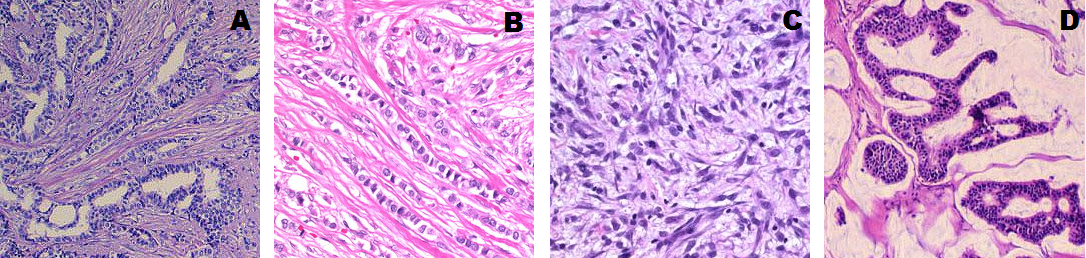
\includegraphics[scale=0.5]{morphology_labelled.png}
            \caption[Breast carcinoma invasive morphologies/histologies.]{Breast carcinoma invasive morphologies/histologies. (A) Ductal, (B) Lobular, (C) Metaplastic, (D) Mucinous. Images taken from \cite{Ramnani2016Webpathology.com:Images, Abdelmessieh2016BreastOverview}}
            \label{fig:histology}
            \end{figure} 
    
  IDC and ILC have distinct pathological features. Specifically, lobular carcinoma small cells are arranged individually, in single sheet pattern, and they have different molecular and genetic aberrations that distinguish them from ductal carcinomas \cite{weigelt2010molecular}. The lobular phenotype is determined by dyregulation of cell-cell adhesion, primarily driven by lack of \textit{E}-cadherin protein expression, which is often used as staining marker to tell it apart from the ductal morphology \cite{Abdelmessieh2016BreastOverview, Ciriello2015ComprehensiveCancer}. Ductal carcinoma has no specific histological characteristics other than invasion through the basement membrane of a breast duct \cite{Weigelt2008RefinementTypes}. 
   
    Metaplastic and mucinous carcinomas are very rare types of breast carcinomas that account for $>1\%$ and $2\%$ of all cases  \cite{Makki2015DiversityRelevance}. 
    Metaplastic breast cancer is a histologically distinct type due to its characteristic outlook of complex admixture of differentiated cells  \cite{Makki2015DiversityRelevance}. It is made up of abnormally looking ductal-origin cells which are thought to have undergone a change in form (\textit{metaplasia}) to become completely different cells that look like soft and connective tissue in the breast. Metaplastic breast cancers are also known to  behave more aggressively than other kinds of breast cancers \cite{schwartz2013metaplastic}. 
    It has been show that $>90\%$ of these cancers lack expression of ER/PR and HER2 (i.e. triple negative), and display a basal-like molecular profile \cite{Weigelt2010a} (more details in the following sections).


    Mucinous carcinoma is less aggressive than more typical kinds of invasive cancer. The histological hallmark of this carcinoma is the excess of extracellular mucin, which surrounds the cancer cells and becomes a part of the tumour \cite{dumitru2015mucinous}.  Mucinous tumours are usually ER/PR positive and HER2 negative, and consistently display a luminal phenotype \cite{Weigelt2010a}. 
    

   
    \subsubsection{Receptor Status}
    
    The identification of breast cancer receptor status is routinely used for prognostic and predictive  purposes \cite{Zaha2014}. A prognostic factor aims to give an indication of patient's overall clinical outcome (i.e. risk of recurrence and mortality), while a predictive factor is any measurement associated with response to a given therapy \cite{cianfrocca2004prognostic}. 
    
    The most common method of testing for receptor status is immunohistochemistry (IHC), which stains the cells based on the presence of estrogen receptors (ER), progesterone receptors (PR) and  human epidermal growth factor receptor 2 (HER2) \cite{Zaha2014}. Receptor status is a critical assessment for all breast cancers as it determines the suitability of using targeted adjuvant treatments such as tamoxifen and trastuzumab, which are now one of the most effective treatments of breast cancer \cite{stickeler2011prognostic}. 

    Approximately 70\% of invasive breast cancers are ER and/or PR positive. Estrogen and/or progesterone receptor positive cancer cells depend on estrogen or related hormones for their growth, therefore this kind of cancer can be treated with endocrine therapy drugs to reduce either the effect of estrogen (e.g. tamoxifen) or the actual levels of estrogen itself \cite{early2005effects}. In this way, hormone therapy blocks the tumour from using estrogen and/or progesterone thereby slowing or stopping its growth. 

    15-20\% of invasive breast cancers are characterised by overexpression of HER2  \cite{stickeler2011prognostic}, which is a good example of both a prognostic and predictive biomarker. HER2 expression is associated with a worse prognosis and higher risk of recurrence, however, HER2+ patients can immensely benefit from the highly effective therapeutic option such as the monoclonal antibody therapy (trastuzamab) \cite{iqbal2014human}. 

    Cancers that do not express any of the three receptors (ER, PR, HER2) are referred to as triple-negative breast cancers (TNBC) \cite{foulkes2010triple}. Triple-negative breast cancers comprise a very heterogeneous group of cancers with a variety of prognoses, but most often thay are associated with a more aggressive outlook. These cancers are the most challenging type, because they do not respond to endocrine therapy or other available targeted agents \cite{hudis2011triple}. 

    
    
    
    
    
    
    
            
 
            
    \subsubsection{PAM50 Molecular Profile}
    

With the wider adaptation of high-throughput gene expression profiling, it has been shown that tumour cell response to treatment is determined by ‘molecular profiles’ rather than physiological tumour characteristics and receptor status \cite{Weigelt2010}. 

The original studies by Sørlie \textit{et al.} \cite{Srlie2001GeneImplications} classified breast cancer tumours into five intrinsic subtypes with distinct clinical outcomes based on their ‘molecular portrait’: Luminal A, Luminal B, Basal-like, HER2-enriched, and Normal-like. The classification was guided by the differences underlying the gene expression patterns that reflect the fundamental differences of the tumours at the molecular level \cite{Srlie2003RepeatedSets}. The observed five subtypes map quite well to the previously defined IHC receptor subtypes (Table  \ref{table:pam50summary}), and have been repeated by several other studies with varying number of genes included in the subtypes’ signature \cite{Dai2015}. 

In 2009, Parker \textit{et al. }\cite{ParkerSupervisedSubtypes} reported a clinically applicable 50-gene classifier, PAM50, containing mostly hormone receptor and proliferation-related genes. By comparing global gene expression data from microarray and qRT-PCR, a minimized set of 50 genes was identified that could reliably classify each tumour into one of the intrinsic subtypes with 93\% accuracy. Over the past 7 years, the PAM50 intrinsic subtypes have shown to provide significant prognostic and predictive information beyond standard clinicopathological parameters \cite{GnantPredictingAlone, Vidal2017}. The PAM50 assay is now clinically implemented worldwide using the \textit{nCounter} platform \cite{Vidal2017}.

\begin{table}[!h]
\centering
\caption[Summary of the breast cancer molecular subtypes.]{Summary of the breast cancer molecular subtypes. PAM50 subtypes map to IHC status subtypes. Ki67 proliferative marker is used as a distinction between Luminal A and B. Luminal A and Normal-like share the IHC subtype. \textit{Table adapted from \cite{Dai2015}.}}
\label{table:pam50summary}
\begin{tabular}{l|c|l}
\multicolumn{1}{c|}{\textbf{PAM50  subtype}} & \textbf{IHC receptor status} & \multicolumn{1}{c}{\textbf{Prognosis}} \\ \hline
\multicolumn{1}{|l|}{Luminal A} & {[}ER+PR+{]} HER2-- Ki67-- & \multicolumn{1}{l|}{\textit{Good}} \\ \hline
\multicolumn{1}{|l|}{\multirow{2}{*}{Luminal B}} & {[}ER+PR+{]} HER2-- Ki67+ & \multicolumn{1}{l|}{\textit{Intermediate}} \\ \cline{2-3} 
\multicolumn{1}{|l|}{} & {[}ER+PR+{]} HER2+ Ki67+ & \multicolumn{1}{l|}{\textit{Poor}} \\ \hline
\multicolumn{1}{|l|}{HER2-enriched} & {[}ER--PR--{]} HER2+ & \multicolumn{1}{l|}{\textit{Poor}} \\ \hline
\multicolumn{1}{|l|}{Basal-like} & {[}ER--PR--{]} HER2--, basal marker & \multicolumn{1}{l|}{\textit{Poor}} \\ \hline
\multicolumn{1}{|l|}{Normal-like} & {[}ER+PR+{]} HER2-- Ki67-- & \multicolumn{1}{l|}{\textit{Intermediate}} \\ \hline
\end{tabular}
\end{table}
    

\textbf{Luminal tumours}\\
Luminal A and B subtypes are distinguished by the expression of two main biological processes: proliferation/cell cycle-related pathways and luminal/hormone-regulated pathways \cite{Vidal2017}, and have expression patterns reminiscent of the luminal component of the breast \cite{perou2000molecular}. Luminal tumours are the most common subtypes among breast cancer (~60\%) with Luminal A being the majority \cite{Dai2015}.  Luminal A is characterised by expression of ER-related genes and low expression of proliferative genes \cite{eroles2012molecular}. The IHC profile for Luminal A includes positive expression of ER, PR, cytokeratin CK8/18, and absence of HER2 expression and low Ki67 (proliferation marker) \cite{Vidal2017}. Luminal B tumours have higher expression of proliferation related genes, and lower expression of luminal-related genes or proteins such as PR and FOXA1, but not ER \cite{prat2012prognostic}, which is found similarly expressed between two luminal subtypes and can only help distinguish luminal from non-luminal disease \cite{Vidal2017}.

In general, the luminal subtypes carry a good prognosis, with Luminal B tumours having a significantly worse scenario than the Luminal A \cite{Srlie2003RepeatedSets}. Treatment response differs between the two, but generally they respond well to hormone therapy and poorly to conventional chemotherapy \cite{brenton2005molecular}. Luminal A tumours could be adequately treated with just endocrine therapy, while Luminal B tumors which are more proliferative will benefit more from the combined therapeutic strategy of chemotherapy and hormonal treatment \cite{paik2004multigene}.\\


\textbf{HER2-enriched tumours}\\
The identification of HER2-enriched subtype among the molecular profiles found in breast cancer was reassuring because it confirmed the clinical impression that the tumours with HER2 overexpression are systematically different from other breast cancers \cite{brenton2005molecular}. 
The HER2-enriched subtype is characterised by the high expression of HER2-related and proliferation-related genes, intermediate expression of luminal-related genes, and low expression of basal-related genes and proteins \cite{Vidal2017}. The best mapping IHC subtype to HER2-enriched tumours is HER2-overexpressed  (ER--/PR--/HER+), but it is not exclusive to them, i.e. it can also be associated with other subtypes \cite{Dai2015}. Additionally, although the majority (68\%) of HER2-enriched tumours have HER2 amplification, there are also cases of HER2-enriched subtype with HER2 negative receptor status \cite{Vidal2017}.

HER2-enriched tumours carry poor prognosis that is derived from a higher risk of early relapse \cite{carey2007triple}, but they can benefit greatly targeted therapeutic agents, such as anti-HER2 monoclonal antibody trastuzumab. \\

\newpage
\textbf{Basal-like tumours}\\
The Basal-like subtype name comes from the observation that the expression pattern of this subtype resembles that of the basal epithelial cells in other parts of the body and normal breast myoepithelial cells \cite{perou2000molecular, brenton2005molecular}. The characteristics include lack of expression of ER-related (luminal) genes, low expression of HER2, and strong expression of basal markers (such as cytokeratins 5, 6, 17) \cite{sotiriou2003breast}. Some of the important hallmarks of basal phenotype is low expression of BRCA genes \cite{callagy2003molecular} and aggressive features such as TP53 mutations \cite{Srlie2001GeneImplications}. 

Among all the intrinsic subtypes, Basal-like is the most distinct \cite{TCGAComprehensiveTumors}. The unsupervised results in 2013 study by Prat \textit{et al.} \cite{prat2013genomic}  revealed that a subgroup of breast cancers, Basal-like by PAM50, should be considered a molecular entity by itself just like ovarian or colorectal cancer, and that $>70\%$ of Basal-like breast cancers were more similar to squamous cell lung cancer than to Luminal A or B disease \cite{prat2013genomic}. 

Basal-like tumours account for 60-90\% of triple negative breast cancers \cite{fan2006concordance}, and in the past the terms TNBC and Basal-like were used interchangeably \cite{Vidal2017}. However, within TNBC, all intrinsic molecular subtypes can be identified. 

Triple negative Basal-like tumours are of particular interest because of their aggressive clinical course and currently lack any form of standard targeted systemic therapy. These tumors are associated with a lower disease-specific survival and a higher risk of local and regional relapse \cite{hudis2011triple}. 
The size of basal tumors is, in general, larger than the other subtypes \cite{rakha2006morphological}, and they also tend to show rapid growth \cite{ho2012characterization}. The metastasis pattern also separates basal tumors from the other breast cancers, with its tendency towards internal organs (excluding bone) and less likely to involve lymph nodes \cite{ho2012characterization}. 

The poor prognosis of Basal-like subtype  has been confirmed by multiple independent data \cite{brenton2005molecular}. However, it is not clear if this prognosis is due to poor therapy options or inherent aggressiveness. Given the triple negative receptor status,  basal tumors are not amenable to conventional targeted breast cancer therapies such as endocrine therapy or trastuzumab, leaving chemotherapy the only option \cite{brenton2005molecular, Dai2015}. \\


\textbf{Normal-like tumours }\\
Normal-like intrinsic subtype is the smallest breast cancer group that accounts for less than 10\% of the cases \cite{Dai2015}. Normal-like subtype shares its IHC receptor status with Luminal A ([ER+ PR+] HER2-- Ki67--), but differs on expression pattern. Also, as suggested by the name, Normal-like cancers are characterised by a normal breast tissue profiling \cite{perou2000molecular}. Still, while Normal-like breast cancer carries a good prognosis, it is slightly worse than Luminal A cancer’s prognosis.\\




























    \newpage    
    \subsection{The Cancer Genome Atlas}
    
    
    
    \subsubsection{Purpose and Organisation}

    The Cancer Genome Atlas (TCGA) network \cite{TheTCGA}, a collaboration between the National Cancer Institute (NCI) and National Human Genome Research Institute (NHGRI), and a part of NCI Genomic Data Commons (GDC) portal from 2016 \cite{NCICommons, gdc2016}, maintains a public database of clinical and molecular data over 33 different tumour types with hundreds of cases per type, making it the most comprehensive repository of human cancer data \cite{OverviewTCGA}. Over the past decade TCGA research network has generated and maintained 2.5 petabytes of data describing tumour and matched normal tissues from more than 11,000 patients that is publicly available and has been used widely by the research community \cite{OverviewTCGA}. The data have contributed to more than a thousand studies of cancer by independent researchers and to the TCGA research network publications \cite{Editorial.2015TheGenomics}.

    The structure of TCGA is well organised and involves several cooperating centres responsible for collection and sample processing, followed by high-throughput sequencing and bioinformatics data analyses \cite{OverviewTCGA, Tomczak2015TheKnowledge}. The generated data is made available to the research community through public free-access databases such as NCI GDC data portal, GDC Legacy Archive and the Broad Institute’s Firehose \cite{PapaleoTCGAPackages}. \\To provide comprehensive analysis of cancer genome profiles, the TCGA research network works with many centres utilising different high-throughput platforms to provide global information of cancer genomics. Some of the applied methods include: RNA-sequencing, miRNA-sequencing, exon sequencing, SNP genotyping, DNA methylation profiling, Reverse-phase protein array (RPPA) \cite{OverviewTCGA}. The multidimensional analyses performed on these distinct platforms provide scientists with a better understanding of cancer biology leading to improved cancer classification as well as development of new diagnostic methods and therapeutic approaches.\\



    \subsubsection{Data Access}

    Two versions of TCGA data are available: harmonised and legacy. The harmonised data is accessible via the NCI GDC data portal \cite{NCICommons}, and it represents a subset of the full TGCA data that has been harmonised against GRCh38 (hg38) genome using GDC Bioinformatics Pipelines. The GDC Legacy Archive provides access to an unmodified copy of data that was previously stored in the TCGA Data Portal hosted by the TCGA Data Coordinating Center (DCC), and  which uses as references GRCh37 (hg19) and GRCh36 (hg18) \cite{PapaleoTCGAPackages}.

    The legacy data is provided as different levels that are defined in terms of a specific combination of both processing level (raw, normalised, integrated) and access level (controlled or open access), while the GDC open access data does not require authorisation to access the high level genomic data that is not individually identifiable \cite{NCICommons, PapaleoTCGAPackages}.
    
    Finally, the data provided by GDC data portal and GDC Legacy Archive can be accessed using R/Bioconductor package TCGAbiolinks \cite{Colaprico2016}. The Bioconductor project ensures high-quality, well-documented and interoperable software and the possibility of integration with hundreds of available packages within R, and is a highly valuable bioinformatics resource \cite{gentleman2004bioconductor}. \\TCGAbiolinks aids in querying, downloading, pre-processing, and analysing TCGA within a single package, allowing user to have a better control over the data and ensuring results reproduciblity \cite{Colaprico2016}. The full clinical report and molecular data (quantified by a variety of methods mentioned above) are prepared to be downloaded as a ‘SummarizedExperiment’ object \cite{Huber2015OrchestratingBioconductor}, which allows easy integration with other data types and statistical methods that are common in the Bioconductor repository.  In line with that, the TCGAbiolinks package has a variety of incorporated methodologies for processing and filtering the data.  
    
    \newpage
    \subsubsection{Breast Cancer Dataset}
    
    TGCA breast cancer dataset (TCGA-BRCA) is the largest by the number of patients cancer type dataset available in TCGA. One of the most complete breast cancer characterisation studies that has ever been performed is the 2012 TCGA Research Network study \cite{CancerGenomeAtlasNetwork2012ComprehensiveTumours} that succeeded to identify comprehensive molecular portraits of human breast tumours. 
    
    In this study, around 500 primary breast cancers were extensively profiled at the DNA (i.e., methylation, chromosomal copy number changes, and somatic and germ line mutations), RNA (i.e., miRNA and mRNA expressions), and protein (i.e., protein and phosphorprotein expression) levels using the most recent technologies \cite{CancerGenomeAtlasNetwork2012ComprehensiveTumours, Vidal2017}.
    
    By classifying tumours using each individual platform and comparing results at different levels through combining the data together in a cluster of clusters, they concluded that diverse genetic and epigenetic alterations converge phenotypically into four major breast tumour subgroups \cite{CancerGenomeAtlasNetwork2012ComprehensiveTumours}. But also importantly, these four entities were found to be recapitulated very well by the four main intrinsic subtypes (Luminal A, Luminal B, HER2-enriched, and Basal-like) as previously defined by mRNA expression only in the Parker’s study \cite{ParkerSupervisedSubtypes}. The Normal-like subtype had limited amount of samples, and therefore was not rigorously explored. Overall, these results suggested that intrinsic subtyping captures a great amount of biological diversity that occurs in breast cancer. 
    
    Another large-scale TCGA-BRCA study was conducted by Ciriello \textit{et al.} in 2015 \cite{Ciriello2015ComprehensiveCancer} on profiling 817 breast cancer samples. The study had a much larger proportion of lobular carcinoma tumours than the original TCGA work, where those were underrepresented. The study shed new light on the genetic bases of lobular morphology and provided more insights into the intrinsic subtypes and their distribution across different morphologies. 
    
    
    
   
    
    
    
    




    
    
    
    
    
    
    
    
    
        
        
        
     \newpage   
    \subsection{Autophagy}
    
    \subsubsection{Overview}

    Autophagy is a highly conserved self-degradative process that has a key role in cellular stress adaptation and survival. Cell homeostasis is achieved by balancing biosynthesis and turnover, and autophagy is the main catabolic process responsible for degrading and recycling cytoplasmic organelles and protein aggregates \cite{Feng2015}. The formation of a specialised cargo vesicle for capturing those macromolecules, called autophagosome, is a unique feature of macroautophagy, which is the main focus of this project. 

    Turnover of cytoplasmic content is an essential cellular house-keeping process, so autophagy happens at any given moment in every cell at low, basal levels \cite{levine2008autophagy}. Autophagy is adaptive and tightly-regulated, and it can be rapidly induced by stimulation from various stresses such as nutrient or growth factor deprivation, hypoxia, DNA damage, damaged organelles, or intracellular pathogens \cite{Kroemer2010}. It can be selective or non-selective, depending on the stimulus and cellular context, leading to different outcomes \cite{Feng2015}. Non-selective autophagy is primarily a cytoprotective response to the aforementioned stresses. 
    Besides autophagy, the cellular response to stress involves numerous other pathways including those that regulate nutrient uptake, metabolism, cell cycle and growth control. Therefore, it is not surprising that there is a close integration between signals that regulate those processes and autophagy, and also the fact that autophagy is involved in a variety of different physiological and pathological processes, including inflammation, development, energy homeostasis, cancer, cell survival and cell death \cite{levine2008autophagy}.

    Upon starvation or stress conditions, autophagy is upregulated. Damaged organelles and cytoplasm are sequestered by an expanding phagophore, leading to the formation of double-membrane autophagosome \cite{Feng2015}, as shown in Figure \ref{fig:autophagosome}. The autophagosome subsequently fuses with a lysosome, followed by degradation of the sequestered cargo by resident hydrolases \cite{Yorimitsu2005Autophagy:Self-eating}. Degradation allows cells to eliminate damaged or harmful components through catabolism and recycling. Then, the breakdown products are released back in cytosol through permeases, where they can be reused as building blocks to generate energy to maintain cell viability under unfavourable conditions \cite{Feng2013TheMacroautophagy}. 


            %basic pathway
            \begin{figure}[!h]
            \centering
            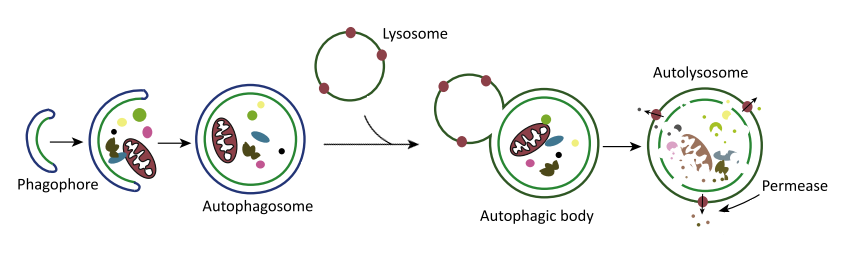
\includegraphics[scale=0.63]{autophagy_mechanism1.png}
            \caption[Overview of autophagosome formation]{Overview of autophagosome formation, with primary membrane structures involved in autophagy depicted. The phagophore is the initial sequestering compartment that expands into a double-membrane autophagosome. Autophagosome fuses with lysosome to initiate degradation of the captured cargo (organelles and damaged proteins). The breakdown products are released to cytosol via permeases for reuse. \textit{Image adapted from \cite{Feng2015}.} }
            \label{fig:autophagosome}
            \end{figure} 
            
    The molecular cascade that regulates and executes autophagy has been the subject of a number of recent, comprehensive reviews \cite{Feng2015, Abada2014}, \cite{ Fullgrabe2016, Kaur2015}, but the full mechanism remains not fully understood. In 2016, Nobel Prize in Physiology or Medicine was given to Prof Yoshinori Ohsumi \cite{The2016}, a renowned scientist in the autophagy research field, for his success in elucidating the sophisticated machinery of the autophagy pathway. The work of Ohsumi and the colleagues has led to identification several dozens of autophagy-related genes, allowing for targeted research aimed at understanding of the autophagy mechanisms \cite{Feng2015}. 

    In the following sections, the overview of autophagosome biogenesis and the brief summary of the main signalling cascades needed for regulation of autophagy are provided. 



        \subsubsection{The Core Pathway of Autophagy }
        
        
      Autophagy is regulated by a set of genes called AuTophaGy-related genes (ATGs). Among them, the group of genes that is essential for autophagosome formation is referred to as the ‘core’ molecular machinery \cite{Xie2007}. These core ATG proteins form three functional complexes:
      \begin{itemize}
          \item the ULK1/2--Atg13--FIP200--Atg101 complex; 
          \item the Beclin-1--class III phosphatidylinositol 3-kinase (PtdIns3K/PI3K) complex; 
          \item two ubiquitin-like protein (Atg12 and LC3) conjugation systems;
    \end{itemize}
    and various proteins that mediate fusion between autophagosomes and lysosomes \cite{Feng2015, Yang2010}. 

    The autophagy core process is divided into mechanistically distinct steps \cite{He2009}, which include induction, elongation and expansion of the phagophore, cargo recognition and selection, vesicle formation, autophagosome maturation via docking and fusion with lysosome/endosome, and breakdown of cargo followed by release of degradation products to cytosol.
    
    The autophagosome formation takes place at the phagophore assembly site (PAS) \cite{kim2002con}, to which most of the core ATG proteins are recruited. The main sign of autophagy initiation is the ULK complex formation. ULK1/2 forms a large complex with the Atg13 gene product and the scaffold protein FIP200, Figure \ref{fig:corepath} (abbreviations in the legend). This happens downstream of the mTOR complex (mammalian target of rapamycin), which is a critical regulator of autophagy induction. 
    
    When mTOR is activated (via Akt and MAPK signalling) it suppresses autophagy, but negative regulation of mTOR (AMPK and p53 signaling) promotes it \cite{Yang2010}. Under nutrient-rich conditions, mTOR is associated with the ULK1/2  and phosphorylates them and Atg13; upon starvation, mTOR disassociates from ULK, which then phosphorylates FIP200 and in this way initiates autophagosome formation \cite{lamb2013}. 
    
        Next, in the nucleation stage, the activated ULK complex targets a class III PI3K complex — consisting of Beclin 1,  VPS34, p150 and Atg14 — to promote the local production of a pool of phosphatidylinositol 3-phosphate that is specific to autophagosomes \cite{Kaur2015}. AMBRA1 mediates ULK dimerisation \cite{Nazio2013MTORTRAF6}, and its interaction with Beclin 1 is regulated by both ULK1 and Bcl-2.        
        

    
    Finally, in the autophagosome expansion stage (Figure \ref{fig:corepath}, bottom left), the Atg12–Atg5–Atg16 complex is recruited to the autophagosome membrane where it facilitates the lipidation of LC3 (also known as MAP1LC3) with phosphatidylethanolamine (PE). The complex formation takes place as follows:  Atg12 is conjugated to Atg5 in a ubiquitin-like reaction that requires Atg7 and Atg10 (E1 and E2-like enzymes, respectively). The Atg12-Atg5 conjugate then interacts noncovalently with Atg16 to form a large complex \cite{He2009}. LC3 is cleaved at its C-terminus by Atg4 protease to generate the cytosolic LC3-I. LC3-I is conjugated to PE also in a ubiquitin-like reaction that requires Atg7 and Atg3 (E1 and E2-like enzymes) \cite{He2009}. The lipidated form of LC3, known as LC3-II, is attached to the autophagosome membrane. The lipidation of LC3 is widely used to monitor autophagy induction. \\
 
        Selective autophagy, which is a targeted engulfment of specific cargos marked with degradation signals, is becoming increasingly appreciated \cite{Kaur2015}. The most studied example is \textit{mitophagy} (Figure \ref{fig:corepath}, top right), which is a process specifically responsible for the removal of dysfunctional mitochondria from the cell.
    Upon mitochondrial damage, the protein PINK, which is continually degraded by PARL under normal conditions, is stabilised and recruits the E3 ligase Parkin (also known as PARK1) to initiate mitophagy \cite{Kroemer2010}. Polyubiquitination of mitochondrial membrane proteins by Parkin results in the recruitment of \textit{autophagy adaptor proteins} SQSTM1/p62, NBR1 (next to BRCA1 gene 1 protein), and AMBRA1. These are the proteins that mediate the targeting of autophagosomes to cargo (in this example, mitochondria) \cite{Kaur2015}. The targeting happens via binding to LC3 via their LC3-interacting region (LIR) and ubiquitin. In addition, BNIP3 and BNIP3L/NIX, which also contain LIRs, directly recruit autophagic machinery by a ubiquitin-independent mechanism to induce autophagosome formation in certain cell types \cite{Kroemer2010}.\\
    
    
     
    % Autophagy and apoptosis are connected both positively and negatively, and extensive crosstalk exists between the two processes. During nutrient deficiency, autophagy functions as a pro-survival mechanism; however, excessive autophagy may lead to cell death, a process morphologically distinct from apoptosis. Several pro-apoptotic signals, such as TNF, TRAIL, and FADD, also induce autophagy. Additionally, Bcl-2 inhibits Beclin-1-dependent autophagy, thereby functioning both as a pro-survival and as an anti-autophagic regulator.
        
                 %core autophagy
             \begin{figure}[!h]
            \centering
            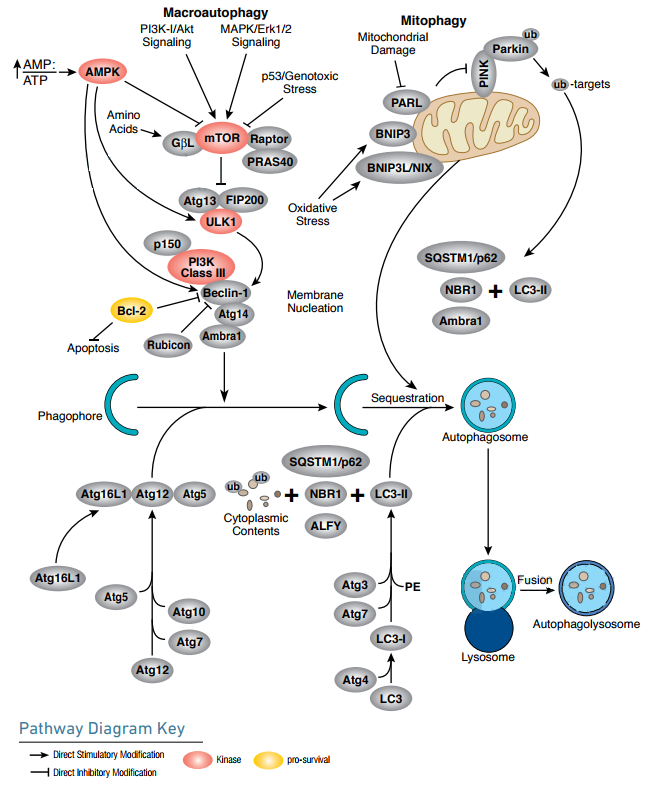
\includegraphics[scale=0.68]{autophagy_mechanism3.png}
            \caption[Autophagy core pathway mechanism]{The core pathway of autophagy regulation. Autophagy is regulated by a complex signaling network of various stimulatory (arrowheads) and inhibitory (bars) inputs. Details in the main text. \textit{Abbreviations:} \textbf{PE} -- phosphatidylethanolamine, \textbf{MAP1LC3}/LC3 -- microtubule-associated protein 1 light chain 3, \textbf{AMBRA1} -- activating molecule in Beclin 1-regulated autophagy 1, \textbf{Bcl-2} -- B cell lymphoma 2, \textbf{VPS} -- vacuolar protein sorting, \textbf{FIP200} -- FAK family kinase interacting protein of 200 kDa, \textbf{mTOR} - mammalian target of rapamycin, SQSTM1 -- sequestosome 1, \textbf{ULK} -- unc-51-like kinase, \textbf{NBR1} -- next to BRCA1 gene 1 protein, \textbf{PINK} -- PTEN induced putative kinase. \textit{Image taken from \cite{AutophagyTechnology}.}
            }
            \label{fig:corepath}
            \end{figure} 

            
            
            
            

    \newpage
    
    \subsubsection{Signalling Pathways Regulating Autophagy}


    As established in the previous section, autophagy initiation is ultimately controlled by mTOR. Its inactivation in response to nutrient depletion results in the activation of the ULK complex and thus the induction of autophagy. The mTOR signalling pathway is critical because of its ability to integrate the information from nutrient, metabolic, and hormonal signals \cite{lamb2013}.  However, hypoxic stimuli can induce autophagy through an mTOR-independent pathway.\\ This section briefly summarises the mTOR-dependent and independent pathways of autophagy initiation. 
    
    Figure \ref{fig:autosignal} presents the signalling regulation of mammalian autophagy. Integration of the main signalling pathways, the class I PtdIns3K signalling and amino acid-dependent signalling, is maintained by mTOR. 
    Insulin has been shown to inhibit autophagy; activation of insulin/growth factor receptor (and its adaptor, IRS1) stimulates the PtdIns3K complex and small GTPase Ras, leading to activation of the PtdIns3K–PKB–TOR pathway \cite{Yang2010}. PKB is activated through PKD1 and phosphorylates and inhibits the tuberous sclerosis complex 1/2 (TSC1–TSC2), leading to the stabilisation of Rheb, which in turn activates mTOR, leading to autophagy inhibition \cite{meijer2004regulation,Yang2010a}.
    
     Amino acids inhibit the Raf-1–MEK1/2–ERK1/2 signalling cascade, causing autophagy inhibition (i.e. nutrient-rich environment). Energy depletion causes AMPK to be phosphorylated and activated by LKB1. AMPK phosphorylates and activates TSC1–TSC2, leading to inactivation of mTOR and autophagy induction. p70S6K kinase is a substrate of mTOR that may negatively feed back on TOR activity, ensuring basal levels of autophagy that are important for homeostasis \cite{Yang2010a}. \\
     Finally, JNK1 and DAPK phosphorylate and disrupt the association of anti-apoptotic proteins, Bcl-2 and Bcl-XL with Beclin 1, which leads to the activation of the Beclin 1-associated class III PtdIns3K complex and mTOR-independent stimulation of autophagy \cite{wei2008jnk1}. 
    
    
    
                % auto signalling
                \begin{figure}[!h]
                \centering
                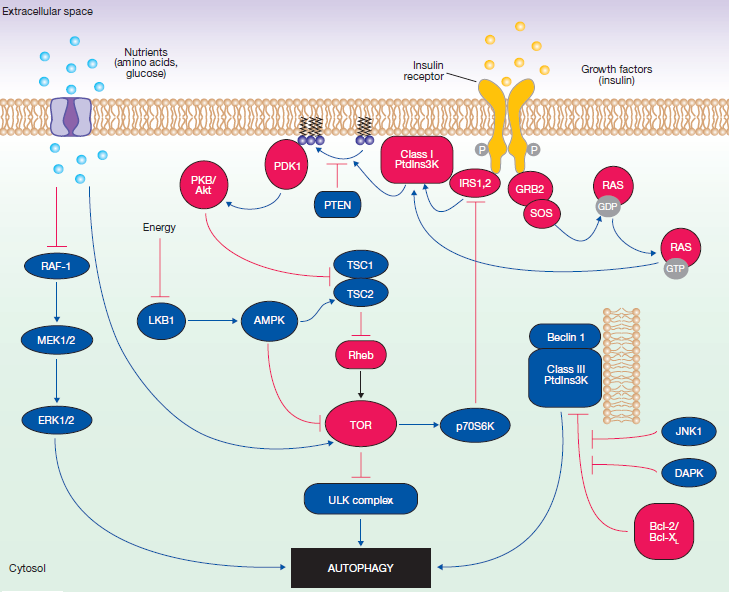
\includegraphics[scale=0.65]{autophagy_signalling.png}
                \caption[Autophagy signalling pathway]{Signalling pathways regulating autophagy. Autophagy is induced by deprivation of nutrients (amino acids), hormones, energy. In the figure, the blue components represent the factors that stimulate autophagy, whereas the red ones correspond to inhibitory factors. Autophagy is regulated by a complex signalling network of various stimulatory (blue arrows) and inhibitory (red bars) inputs.         \textit{Abbreviations:} \textbf{PKB} -- protein kinase B, \textbf{PDK1} -- 3-phosphoinositide-dependent protein kinase 1, \textbf{JNK1} -- c-Jun amino-terminal kinase 1, \textbf{DAPK} -- death-associated protein kinase, \textbf{AMPK} -- AMP-activated protein kinase. 
                \textit{Image taken from \cite{Yang2010a}.}

}
                \label{fig:autosignal}
                \end{figure} 
                
            
            
            
            
            
            
            
            
            
            
            
            
            
            
            
            
            
            
            
            
            
            
        
        
    \newpage    
    \subsection{Autophagy in Cancer}
    % The role of autophagy in tumorigenesis and treatment response is complicated and context-dependent, and presumed to differ between stages of cancer progression (Zarzynska and Magdalena 2014). Autophagy’s role in maintaining organelle and protein turnover allows cells to restrain damage, including genome instability and inflammation, thereby limiting initiation and progression of cancer at early stages. However, once tumour develops, the cancer cells are able to utilize autophagy for their own cytoprotection (Zarzynska and Magdalena 2014). Autophagy is believed to promote cancer by allowing cells to survive under conditions of metabolic and genotoxic stress (Mathew and White n.d.). Unfavourable conditions such as hypoxia and acidity in tumour environment as well as the effects of chemo- and radiotherapy cause cells to experience stress and nutrient deprivation (Bailey et al. n.d.). Induction of autophagy within these cells allows them to survive the drastic conditions. This kind of mechanism had been referred to as “what doesn’t kill you, makes you stronger” by researchers in the field (Mathew and White n.d.).
        \subsubsection{a}
        \subsubsection{b}
        
        
        


\section{Thesis objectives}
